\documentclass[a4paper]{article}

\usepackage{enumerate}
\usepackage{amsmath}
\usepackage{hyperref}
\usepackage[all]{hypcap}
\usepackage{xfrac}

\title{Assignment 1}
\author{Jacco Spoelder (s1348493) \and Xeryus Stokkel (s2332795)}

\begin{document}

\maketitle

\section{Top 500 list}
The end of (one of) our student numbers is 93. At the 93th positon in the current high performance computer top 500 list, as of November 2014, is the SANAM Supercomputer, located in Saudi Arabia. It appeared first in the top 500 list at the end of 2012. It was built by and hosted in the King Abdulaziz City for Science and Technology(KACST) in cooperation with Frankfurt Institute for Advanced Studies(FIAS). At the time it was completed, it ranked the worlds second most efficient supercomputer, based on the performance/energy use ratio. This efficiency is expressed as the computing power in floating point operation per second(FLOPS) per watt of energy used. The SANAM supercomputer is able to do 2,351.10 mega FLOPS per watt. Nowadays it is ranked number 23. The most efficient supercomputer at this moment, the GSI Helmholtz Center based L-CSC, performs 5,271.81 mega FLOPS per watt, more than twice as efficient. At the time of completion the SANAM placed at position 52 in the top 500 supercomputer list, while, as said, it now has position 93. 

The high efficiency and total computing power of the SANAM system is acquired through the use of many general purpose graphic processing units(GPGPU) instead of only central processing units(CPU).
\subsection{Structure}
The structure of the SANAM supercomputer is based on GPU`s. It has 256 server modules, each module consisting of 2 Xeon E5−2650 (2.0 GHz) CPU`s and 2 AMD FirePro S10000 GPU`s. The Xeon E5−2650 CPU`s each have 8 hyperthreading enabled cores and the FirePro S10000 GPU`s have two GPU cores each. Each module harbours 128 GiB DDR3-DRAM of main memory. Benchmarking and testing shows that, for feeding the GPU`s of the system, the 8-core Intel CPU is more efficient than a 6-core CPU with higher clock frequency and comparable performance(Rorh et al 2014).


\section{Speedup}
\begin{enumerate}[(a)]
	\item Speed up is the decrease in time required to solve a problem when using multiple parallel processors. It is defined as
		\begin{equation}
			S(p) = \frac{t_1}{t_p} \label{eqn:base}
		\end{equation}
		where $t_1$ is the time required to solve the problem on a single processor and $t_p$ is the time required to solve the problem on $p$ processors.
	\item Any program can be split up in a part that can be parallised ($t_\text{par}(1)$) and a part which can not ($t_\text{seq}(1)$). We can then define $t_1$ and $t_p$ as follows:
		\begin{align*}
			t_1 &= t_\text{seq}(1) + t_\text{par}(1) \\
			t_p &= t_\text{seq}(1) + \frac{t_\text{par}(1)}{p}
		\end{align*}
		This can be combined with the \autoref{eqn:base} to form:
		\begin{align}
			S(p) &= \frac{t_\text{seq}(1) + t_\text{par}(1)}{t_\text{seq}(1) + \frac{t_\text{par}(1)}{p}} \nonumber \\
			S(p) &= \frac{\frac{t_\text{seq}(1)}{t_\text{par}(1)} + 1}{\frac{t_\text{seq}(1)}{t_\text{par}(1)} + \frac{1}{p}} \label{eqn:step2}
		\end{align}
		\autoref{eqn:step2} contains the ratio $\displaystyle \frac{t_\text{seq}(1)}{t_\text{par}(1)}$, of which we can take the inverse to get the desired ratio $\displaystyle x = \frac{t_\text{par}(1)}{t_\text{seq}(1)}$ so we can rewrite it as follows:
		\begin{align*}
			S(p) &= \frac{x^{-1} + 1}{x^{-1} + p^{-1}}
		\end{align*}
	\item To get the value of the ratio $x$ we need to solve the following:
		\begin{align*}
			\frac{x^{-1} + 1}{x^{-1} + 300^{-1}} &= 200 \\
			x^{-1} + 1 & = 200 (x^{-1} + 300^{-1}) \\
			x^{-1} + 1 &= 200 x^{-1} + \sfrac{2}{3} \\
			199 x^{-1} &= \sfrac{1}{3} \\
			x^{-1} &\approx \sfrac{1}{597} \\
			x &\approx 597
		\end{align*}
	\item Since $S(p) \approx x$ for $p \gg x$ the maximum speed-up is about 600. For example we could use $10^9$ processors: $\displaystyle S(10^9) = \frac{597^{-1} + 1}{597^{-1} + (10^9)^{-1}} \approx 598$, as we can see the speed-up with such a large number of processors is still a bit shy of 600.
	\item To achieve half of the maximum speed up we would need to solve $S(p) = 300$:
		\begin{align*}
			\frac{597^{-1} + 1}{597^{-1} + p^{-1}} &= 300 \\
			300 (597^{-1} + p^{-1}) &= 597^{-1} + 1 \\
			\frac{300}{p} + \frac{1}{2} &= 597^{-1} + 1 \\
			\frac{300}{p} &= \frac{1}{2} + 597^{-1} \\
			p &\approx 598
		\end{align*}
		So 598 processors are needed to get half of the maximum speed-up. This is about the same as the ratio $x$, this means that when there is a processor for each parallelizable part and one extra for the sequential part that about half of the theoretical maximum speed-up can be achieved.
\end{enumerate}

\section{Amdahl's and Gustafson's law}
\subsection{Amdahl's law}
Amdahl's law states that the maximal achievable speed-up is proportional to the parts of the program that cannot be made parallel. Or in other words: the sequential part of the program limits the achievable speed-up. Amdahl's law can be expressed as follows: $S(n) = B + \frac{1 - B}{n}$ where $B$ is the fraction of the program that cannot be parallelized and $n$ is the number of processors.

The law is related to the law of diminishing returns in economics. This law states that the more you invest in improving something, the smaller the effect of an additional investment would be. The same is true for Amdahl's law, if you already have a number of processors then adding extra processors will not give an equal amount of speed-up. So doubling the amount of processors doesn't double the speed-up.

Amdahl's law only describes speed-up in terms of the parallelizable part of a program and the amount of processors that can be used. It does not take thing like memory or other possible bottlenecks into account. The law also only works when datasets do not increase, so the total amount of work stays the same while the number of processors does change.

\subsection{Gustafson`s law}
Compared to Amdahl`s law, which assumes a fixed problem size, Gustafson`s law approaches the parallelization speed-up differently. Amdahl states that the serial portion of the problem does not change iwth an increasing number of processors, so the total speed-up is limited strongly by this serial part, despite the speed-up of the parallel part.
Gustafson law or approach states that with an increasing number of processors, the relative parallel part of the problem also increases. This being especially so with scientific types of problems. If more processors are available, the users tend to increase the computational load. Therefore, the speedup scales far better with the problem size. This is illustrated in \autoref{fig:gustafsonslaw}.

\begin{figure}
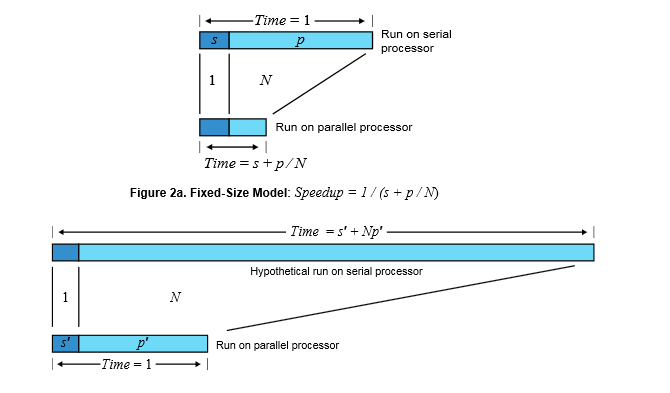
\includegraphics[width=\textwidth]{Law}
\caption{Comparison between Amdahl`s law and Gustafson`s law woth increased problem size. Adapted from Gustafson, 1988.}
\label{fig:gustafsonslaw}
\end{figure}

\pagebreak
\nocite{*}
\bibliographystyle{plain}
\bibliography{assignment1.bib}

\url{http://www.futurechips.org/thoughts-for-researchers/parallel-programming-gene-amdahl-said.html} \\
\url{https://en.wikipedia.org/wiki/Amdahl's_law}
\end{document}